\documentclass[UTF8,fontset=none,12pt]{ctexart}

\setCJKmainfont{Songti SC}
\setCJKsansfont{PingFang SC}
\setCJKmonofont{Songti SC}

\usepackage[a4paper,margin=2.35cm]{geometry}
\usepackage{amsmath,amssymb,amsthm,mathtools,bm}
\usepackage{graphicx}
\usepackage{float}
\usepackage{booktabs}
\usepackage{array}
\usepackage{enumitem}
\usepackage[hidelinks]{hyperref}

\title{数值线性代数\quad 第 35 讲：GMRES}
\author{Lloyd N. Trefethen、David Bau III\quad 中文阅读版}
\date{}

\begin{document}
\maketitle
\pagestyle{plain}

上一讲展示了 Arnoldi 过程如何寻找特征值。本讲说明，同一个过程还可以用来
求解线性方程组 $Ax=b$。这一类方法中最标准的算法称为 GMRES，是
\emph{generalized minimal residuals}（广义最小残量）的缩写。

\section*{在 Krylov 子空间中最小化残量}

和前两讲一样，设 $A\in\mathbb C^{m\times m}$，$b\in\mathbb C^m$，并令

\[
\mathcal K_n=\operatorname{span}\{b,Ab,\ldots,A^{n-1}b\}
\]

为式（33.5）中的 Krylov 子空间。不过现在假设 $A$ 非奇异，因为我们的目标是
求解 $Ax=b$。记精确解为

\[
x_* = A^{-1}b.
\]

GMRES 的核心思想可以用一句话概括：在第 $n$ 步，从 $\mathcal K_n$ 中选取使
残量

\[
r_n=b-Ax_n
\]

的范数最小的向量 $x_n$，即

\[
x_n\in\mathcal K_n,\qquad
\lVert r_n\rVert=\lVert b-Ax_n\rVert=\min.
\]

这就是一个最小二乘问题，图 35.1 给出了它的几何图像。

\begin{figure}[H]
\centering
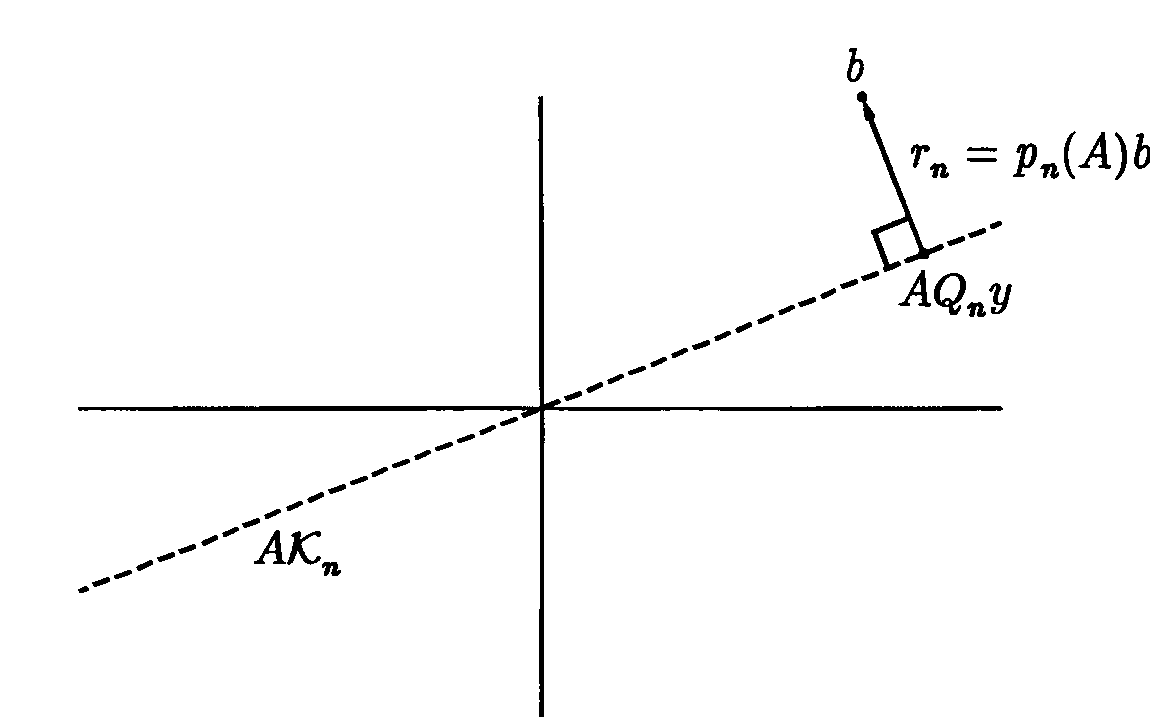
\includegraphics[width=0.78\textwidth]{../assets/figure-35-gmres-least-squares.png}
\parbox{0.78\textwidth}{\small 图 35.1. GMRES 背后的最小二乘多项式逼近问题：最小化残量范数 $\lVert r_n\rVert$。图中的 $AQ_ny$ 是可行近似，$r_n=p_n(A)b$ 是正交残量。}
\end{figure}

一种显然的做法是直接使用 Krylov 矩阵。设 $K_n$ 是 $m\times n$ 的 Krylov
矩阵（式（33.6）），则

\begin{equation}
AK_n=
\begin{bmatrix}
Ab&A^2b&\cdots&A^nb
\end{bmatrix}.
\tag{35.1}
\end{equation}

这个矩阵的列空间就是 $A\mathcal K_n$。于是我们需要寻找 $c\in\mathbb C^n$，
使得

\begin{equation}
\lVert AK_nc-b\rVert=\min,
\tag{35.2}
\end{equation}

其中本书这一部分始终使用二范数。求出 $c$ 后，再令 $x_n=K_nc$ 即可。这个
过程可以通过对 $AK_n$ 做 QR 分解来实现。

然而，上述做法在数值上不稳定，而且会构造一个实际上并不需要的因子 $R$。
实际算法改用 Arnoldi 迭代（算法 33.1）构造一系列 Krylov 矩阵 $Q_n$，其列
向量 $q_1,q_2,\ldots$ 张成相应的 Krylov 子空间。于是写成
$x_n=Q_ny$，而不是 $x_n=K_nc$。最小二乘问题变为寻找 $y\in\mathbb C^n$，
使得

\begin{equation}
\lVert AQ_ny-b\rVert=\min.
\tag{35.3}
\end{equation}

表面上，式（35.3）似乎是一个 $m\times n$ 的问题；但由于 Krylov 子空间的
特殊结构，它实际上只涉及一个 $(n+1)\times n$ 的问题。根据式（33.3），有

\begin{equation}
\lVert Q_{n+1}\widetilde H_ny-b\rVert=\min.
\tag{35.4}
\end{equation}

现在，范数中的两个向量都属于 $Q_{n+1}$ 的列空间，因此左乘
$Q_{n+1}^*$ 不会改变范数。于是问题等价于

\begin{equation}
\lVert \widetilde H_ny-Q_{n+1}^*b\rVert=\min.
\tag{35.5}
\end{equation}

根据 Krylov 矩阵的构造，

\[
Q_{n+1}^*b=\lVert b\rVert e_1,
\qquad e_1=(1,0,0,\ldots)^*.
\]

最终得到 GMRES 的最小二乘形式：

\begin{equation}
\left\lVert \widetilde H_ny-\lVert b\rVert e_1\right\rVert=\min.
\tag{35.6}
\end{equation}

第 $n$ 步先解这个问题得到 $y$，再设置 $x_n=Q_ny$。

\section*{GMRES 的算法结构}

上面的推导已经完成了 GMRES 算法。其高层描述如下。

\begin{center}
\fbox{\begin{minipage}{0.86\textwidth}
\textbf{算法 35.1\quad GMRES}

\[
q_1=b/\lVert b\rVert.
\]

\begin{enumerate}[leftmargin=2.4em,itemsep=0pt]
\item 对 $n=1,2,3,\ldots$：
\begin{enumerate}[label=\arabic*.,leftmargin=2.4em,itemsep=0pt]
\item 执行 Arnoldi 迭代算法 33.1 的第 $n$ 步；
\item 求 $y$，使
\[
\left\lVert \widetilde H_ny-\lVert b\rVert e_1\right\rVert
\]
最小（这个最小值就是 $\lVert r_n\rVert$）；
\item 令 $x_n=Q_ny$。
\end{enumerate}
\end{enumerate}
\end{minipage}}
\end{center}

在每一步，GMRES 都是在所有 $x_n\in\mathcal K_n$ 中最小化残量
$r_n=b-Ax_n$ 的范数。求解 $y$ 的同时就已经得到 $\lVert r_n\rVert$，不必
再根据 $x_n$ 显式计算一次残量。

算法 35.1 中的内部步骤是一个带 Hessenberg 结构的
$(n+1)\times n$ 矩阵最小二乘问题。利用 Lecture 11 中介绍的 QR 分解，可以
以 $O(n^2)$ 次浮点运算求解；Hessenberg 结构正是使这个复杂度成立的原因。
还可以进一步节省工作量：不必每一步都独立地构造
$\widetilde H_1,\widetilde H_2,\ldots$ 的 QR 分解，而是从上一步的分解更新到
这一步。每次只需一个 Givens 旋转（习题 10.4）和 $O(n)$ 的工作量，见习题
35.4。

\section*{GMRES 与多项式逼近}

上一讲说明，Arnoldi 迭代计算特征值与如下逼近问题有关：在首一多项式空间
$\mathcal P^n$ 中寻找 $p^n$，使 $\lVert p^n(A)b\rVert$ 最小。GMRES 也在
解决一个多项式逼近问题，区别在于现在使用的多项式空间是

\begin{equation}
\mathcal P_n=
\{p:\ p\text{ 的次数不超过 }n,\ p(0)=1\}.
\tag{35.7}
\end{equation}

用多项式系数表示时，现在的归一化条件是 $c_0=1$，而不是 $c_n=1$。
记号也从上标改为下标，以提醒读者：归一化点已经从 $z=\infty$ 改为
$z=0$。

GMRES 的迭代向量可以写成

\begin{equation}
x_n=q_n(A)b,
\tag{35.8}
\end{equation}

其中 $q_n$ 是次数为 $n-1$ 的多项式。相应的残量为

\[
r_n=b-Ax_n
=(I-Aq_n(A))b.
\]

令

\[
p_n(z)=1-zq_n(z),
\]

就有

\begin{equation}
r_n=p_n(A)b,
\tag{35.9}
\end{equation}

且 $p_n\in\mathcal P_n$。GMRES 选择 $p_n$ 的系数来最小化该残量的范数。
因此，GMRES 逐步解决如下逼近问题：

\begin{center}
\fbox{\begin{minipage}{0.86\textwidth}
\textbf{GMRES 逼近问题\quad}
寻找 $p_n\in\mathcal P_n$，使得
\[
\lVert p_n(A)b\rVert=\min.
\tag{35.10}
\]
\end{minipage}}
\end{center}

\subsection*{不变性}

GMRES 和 Arnoldi 迭代一样满足一些不变性。下面的定理直接由式（35.10）得到。

\textbf{定理 35.1.}
将 GMRES 迭代应用于 $A\in\mathbb C^{m\times m}$。

\begin{description}[leftmargin=3.55cm,style=sameline]
\item[尺度不变性]
若 $A$ 变为 $\sigma A$，其中 $\sigma\in\mathbb C$，同时 $b$ 变为
$\sigma b$，则残量序列 $\{r_n\}$ 变为 $\{\sigma r_n\}$。

\item[酉相似变换下的不变性]
若 $A$ 变为 $UAU^*$，其中 $U$ 是酉矩阵，同时 $b$ 变为 $Ub$，则按照
残量定义，残量序列变为 $\{Ur_n\}$。
\end{description}

这里第二条按残量的直接变换
\[
Ub-(UAU^*)(Ux_n)=U(b-Ax_n)=Ur_n
\]
写出。原书此处排印为 $\{U^*r_n\}$；这与上述变换及残量定义不一致，
本译稿按定义作了校正。

GMRES 不具有平移不变性，因为归一化条件 $p(0)=1$ 依赖于平移相关的点
$0$。换句话说，GMRES 的行为强烈依赖原点的位置；宽泛地说，它依赖于矩阵
$A$ 的条件数。

\section*{GMRES 的收敛}

GMRES 收敛得有多快？需要多少步，才能把 $\lVert r_n\rVert/\lVert b\rVert$
降到 $10^{-3}$ 或 $10^{-16}$ 这样的水平？在实践中，这个问题往往最终转化
为如何设计一个好的预条件器（见第 40 讲）。从数学上说，我们要研究的是
$A$ 的哪些性质决定了 $\lVert r_n\rVert$ 的大小。

首先有两个观察。第一，GMRES 单调收敛：

\begin{equation}
\lVert r_{n+1}\rVert\leq\lVert r_n\rVert.
\tag{35.11}
\end{equation}

原因是 $\lVert r_n\rVert$ 已经是在 $\mathcal K_n$ 上能够达到的最小值；
把 $\mathcal K_n$ 扩大为 $\mathcal K_{n+1}$ 只会使最小残量范数下降，或至多
保持不变。注意 $\mathcal P_n\subset\mathcal P_{n+1}$，而首一多项式空间
$\mathcal P^n$ 并不包含于 $\mathcal P^{n+1}$。

第二，在没有舍入误差时，至多经过 $m$ 步，过程必须收敛：

\begin{equation}
\lVert r_m\rVert=0.
\tag{35.12}
\end{equation}

对一般的 $A$ 和 $b$，这是因为 $\mathcal K_m=\mathbb C^m$；在特殊情况下，
如果 $b$ 在某个 $n<m$ 时就已经属于 $\mathcal K_n$，则会更早收敛。式
（35.12）有助于记住 GMRES 的数学性质，但实际意义有限：如果一个 GMRES
迭代要有用，就必须在 $n\ll m$ 的步数内达到满意精度。

要得到更有用的收敛信息，需要回到式（35.10）。由最小性可知

\[
\lVert r_n\rVert=\lVert p_n(A)b\rVert
\leq \lVert p_n(A)\rVert\,\lVert b\rVert
\]

对所有 $p_n\in\mathcal P_n$ 都成立。因此，除非右端项 $b$ 具有与 $A$ 的特殊
结构，决定残量大小的关键因素通常是 $\lVert p_n(A)\rVert$。一般有

\begin{equation}
\frac{\lVert r_n\rVert}{\lVert b\rVert}
\leq
\inf_{p_n\in\mathcal P_n}\lVert p_n(A)\rVert.
\tag{35.13}
\end{equation}

于是问题变成：给定矩阵 $A$ 和整数 $n$，$\lVert p_n(A)\rVert$ 能够有多小？
这正是几乎所有线性方程组 Krylov 子空间迭代收敛分析的基础。

\section*{在谱上较小的多项式}

给定 $A$ 和 $n$，估计 $\lVert p_n(A)\rVert$ 的标准方法，是寻找在 $A$ 的谱
$\Lambda(A)$ 上尽可能小、同时满足 $p(0)=1$ 的多项式。若 $p$ 是多项式、
$S$ 是复平面中的集合，定义标量范数

\begin{equation}
\lVert p\rVert_S=\sup_{z\in S}\lvert p(z)\rvert.
\tag{35.14}
\end{equation}

假设 $A$ 可对角化，即

\[
A=V\Lambda V^{-1},
\]

其中 $V$ 非奇异，$\Lambda$ 为对角矩阵。于是

\begin{equation}
\begin{aligned}
\lVert p(A)\rVert
&=\lVert Vp(\Lambda)V^{-1}\rVert\\
&\leq \lVert V\rVert\,\lVert p(\Lambda)\rVert\,\lVert V^{-1}\rVert\\
&=\kappa(V)\,\lVert p\rVert_{\Lambda(A)}.
\end{aligned}
\tag{35.15}
\end{equation}

结合式（35.13），得到 GMRES 收敛性的基本定理。

\textbf{定理 35.2.}
在 GMRES 的第 $n$ 步，残量满足

\begin{equation}
\frac{\lVert r_n\rVert}{\lVert b\rVert}
\leq
\inf_{p_n\in\mathcal P_n}\lVert p_n(A)\rVert
\leq
\kappa(V)\inf_{p_n\in\mathcal P_n}
\lVert p_n\rVert_{\Lambda(A)}.
\tag{35.16}
\end{equation}

这里 $\Lambda(A)$ 表示 $A$ 的特征值集合，$V$ 是特征向量矩阵（假设 $A$
可对角化），$\kappa(V)$ 是 $V$ 的条件数，$\lVert p\rVert_{\Lambda(A)}$
按式（35.14）定义。

这一定理可以用一句话概括：如果 $A$ 不太偏离正规矩阵，即 $\kappa(V)$
不太大；并且能够找到在 $\Lambda(A)$ 上迅速变小的、满足 $p(0)=1$ 的
次数不超过 $n$ 的多项式，那么 GMRES 就会快速收敛。

\section*{例 35.1：良好谱分布下的快速收敛}

考虑一个 $200\times200$ 的矩阵 $A$，其元素相互独立，服从均值为 $2$、
标准差为 $0.5/\sqrt{200}$ 的实正态分布。MATLAB 中可以写成

\begin{equation}
m=200,\qquad
A=2I+0.5\,\operatorname{randn}(m)/\sqrt m.
\tag{35.17}
\end{equation}

图 35.2 给出了 $A$ 的特征值。它们大致均匀地分布在以 $z=2$ 为中心、
半径为 $1/2$ 的圆盘中。

\begin{figure}[H]
\centering
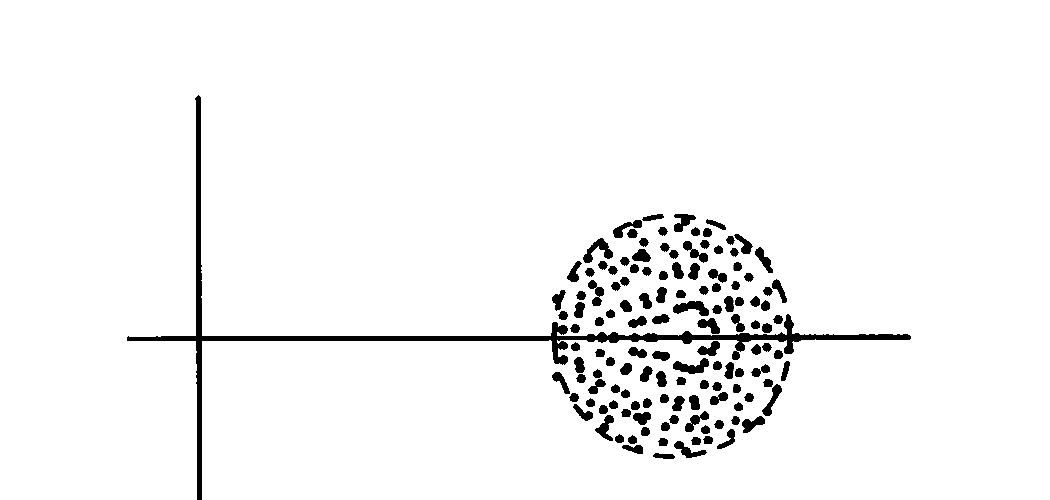
\includegraphics[width=0.72\textwidth]{../assets/figure-35-eigenvalues.png}
\parbox{0.82\textwidth}{\small 图 35.2. 式（35.17）中 $200\times200$ 矩阵 $A$ 的特征值。虚线圆的中心为复平面中的 $z=2$，半径为 $1/2$；特征值大致均匀分布在圆盘内。}
\end{figure}

令 $b=(1,1,\ldots,1)^*$，对 $Ax=b$ 应用 GMRES。图 35.3 给出了收敛曲线，
其速率近似为 $4^{-n}$。原因并不难看出：既然谱大致填满图 35.2 所示的圆盘，
使 $\lVert p(A)\rVert$ 较小的自然选择是

\[
p(z)=\left(1-\frac z2\right)^n.
\]

矩阵 $I-A/2$ 的谱大致填满以原点为中心、半径为 $1/4$ 的圆盘，因此
$\lVert p(A)\rVert$ 大约按 $4^{-n}$ 衰减。这个矩阵条件良好，
$\kappa(A)\approx2.03$；它偏离正规矩阵的程度也不大，特征向量矩阵满足
$\kappa(V)\approx141$。

\begin{figure}[H]
\centering
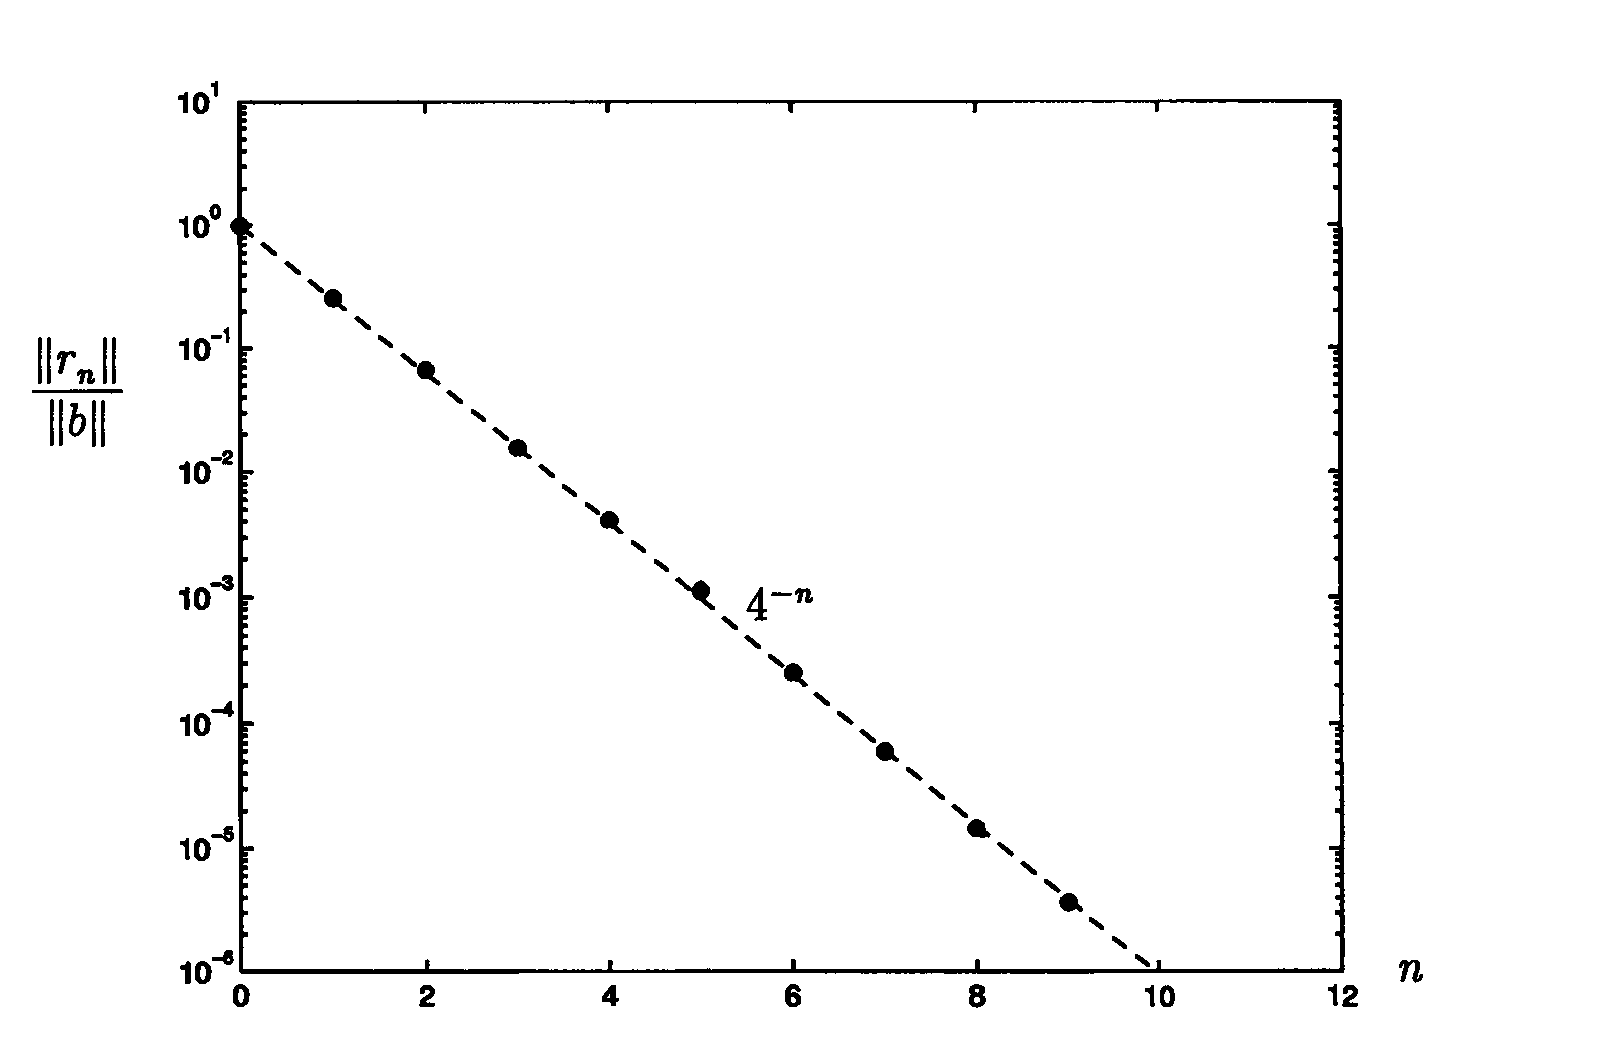
\includegraphics[width=0.90\textwidth]{../assets/figure-35-convergence-good.png}
\parbox{0.90\textwidth}{\small 图 35.3. 同一个矩阵 $A$ 的 GMRES 收敛曲线。快速而稳定的收敛说明：当矩阵性质良好（或已经经过良好预条件化）时，Krylov 子空间迭代可以表现得非常理想。}
\end{figure}

图 35.3 展示了有利条件下的矩阵迭代。十步迭代后即可达到六位数字的精度，
代价约为

\[
10\times 2m^2\approx 8.0\times10^5
\]

次浮点运算，因为主要工作是每一步的矩阵--向量乘法。对同一个系统使用
高斯消元则约需

\[
\frac23m^3\approx5.3\times10^6
\]

次浮点运算。即使 $A$ 没有可利用的稀疏性、维数也只有 $m=200$，GMRES
仍然带来了接近 $7$ 倍的改进。若 $m=2000$，这个倍数大约会达到 $70$；
如果一个 $2000\times2000$ 的矩阵具有相似的谱性质，同时稀疏度为 $90\%$
或 $99\%$，改进倍数还可能达到约 $700$ 或 $7000$，而 GMRES 所需的存储量
也会显著下降。

\section*{例 35.2：谱包围原点时的停滞}

如果矩阵的特征值“包围原点”，就不能期待上述快速收敛。令 $A$ 仍为例
35.1 中的矩阵，定义

\[
A'=A+D,
\]

其中 $D$ 是对角矩阵，其复对角元为

\[
d_k=(-2+2\sin\theta_k)+\mathrm{i}\cos\theta_k,
\qquad
\theta_k=\frac{k\pi}{m-1},
\quad 0\leq k\leq m-1.
\]

如图 35.4 所示，新的特征值形成一片弯向原点的半圆形谱云。

\begin{figure}[H]
\centering
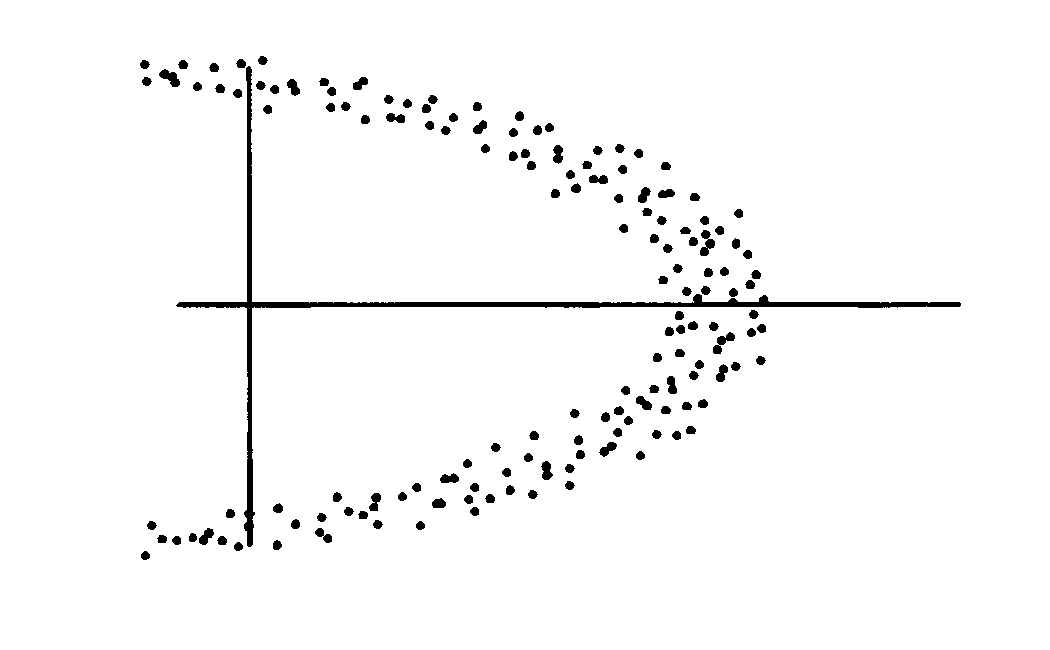
\includegraphics[width=0.72\textwidth]{../assets/figure-35-eigenvalues-bad.png}
\parbox{0.82\textwidth}{\small 图 35.4. 一个与式（35.17）类似、但修改了对角元的 $200\times200$ 矩阵的特征值。现在特征值在一侧围绕原点分布。}
\end{figure}

此时 GMRES 的收敛明显变慢，对于这个问题，迭代计算并不比高斯消元更好。
条件数现在约为 $\kappa(A)\approx4.32$，$\kappa(V)\approx54.0$。因此，收敛
恶化不能只用条件数解释；真正造成困难的是特征值的位置，而不是特征值的
大小（也不是奇异值的大小）。如果这段谱弧继续向另一侧延伸、更加包围谱，
收敛还会进一步变差。

\begin{figure}[H]
\centering
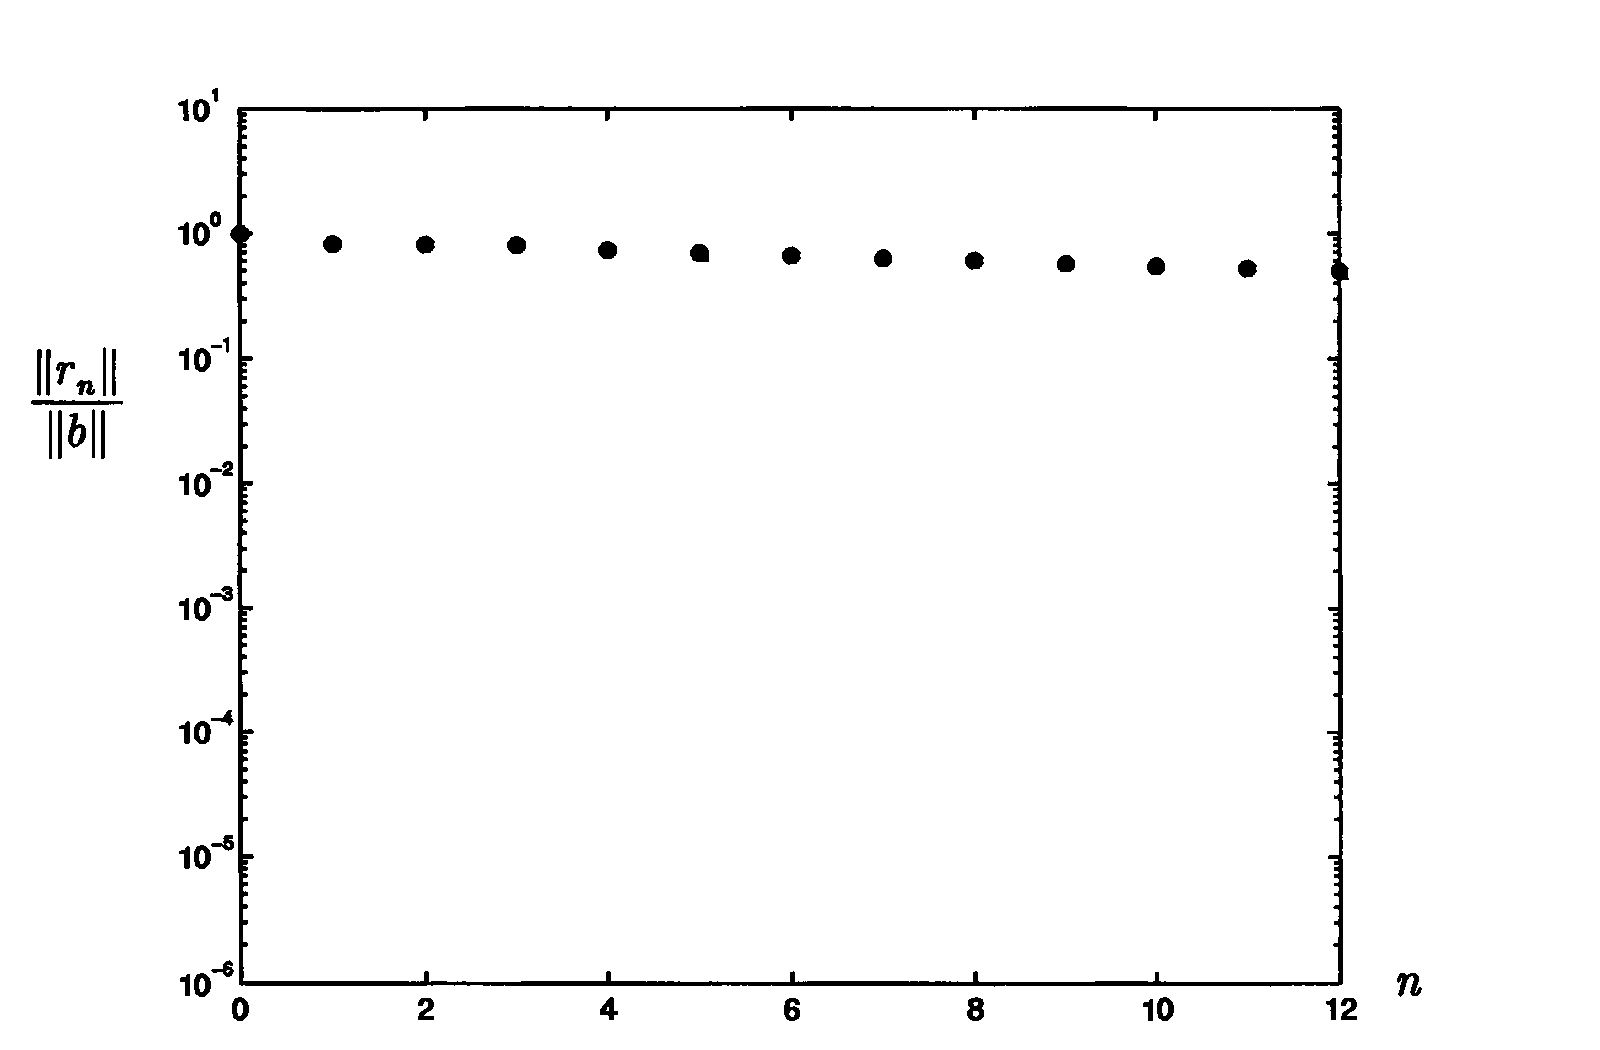
\includegraphics[width=0.90\textwidth]{../assets/figure-35-convergence-bad.png}
\parbox{0.90\textwidth}{\small 图 35.5. 图 35.4 中矩阵的 GMRES 收敛曲线。收敛速度大幅下降；当迭代方法出现这种停滞时，应当寻找更好的预条件器。}
\end{figure}

\section*{习题}

\paragraph{35.1.}
证明：如果 $S\subset\mathbb C$ 含有无穷多个点，那么式（35.14）在所有复系数
多项式组成的向量空间上定义一个范数。如果 $S$ 只有有限多个点，会出现什么问题？

\paragraph{35.2.}
\begin{enumerate}[label=(\alph*)]
\item 设 $S\subset\mathbb C$，其凸包的内部包含 $0$。也就是说，$S$ 不包含于
任何与原点不相交的半平面中。证明：不存在 $p\in\mathcal P_1$（即满足
$p(0)=1$ 的一次多项式）使 $\lVert p\rVert_S<1$。
\item 设 $A$ 是一个不必正规的矩阵，且其谱 $\Lambda(A)$ 满足（a）的条件。
证明：不存在 $p\in\mathcal P_1$ 使 $\lVert p(A)\rVert<1$。
\item 尽管图 35.5 中的收敛很慢，显然仍有 $\lVert r_1\rVert<\lVert r_0\rVert$。
解释这为何不与（b）矛盾，并描述 GMRES 为了实现
$\lVert r_1\rVert<\lVert r_0\rVert$ 可能找到的 $p_1\in\mathcal P_1$ 具有什么性质。
\end{enumerate}

\paragraph{35.3.}
递推式

\[
x_{n+1}=x_n+\alpha r_n
=x_n+\alpha(b-Ax_n),
\]

其中 $\alpha$ 是标量常数，称为 Richardson 迭代。
\begin{enumerate}[label=(\alph*)]
\item 第 $n$ 步对应的多项式 $p(A)$ 是什么？
\item 对图 35.2 中的矩阵 $A$，推荐选择什么 $\alpha$？相应的收敛速率
预计是多少？
\item 对图 35.4 中的矩阵，回答同样的问题。
\end{enumerate}

\paragraph{35.4.}
\begin{enumerate}[label=(\alph*)]
\item 描述一种基于 Givens 旋转 QR 分解的 $O(n^2)$ 算法，用于求解算法 35.1
中的最小二乘问题（见习题 10.4）。
\item 如果第 $n-1$ 步的问题已经求解，说明如何像第 268 页所述，将运算量
改进到 $O(n)$。
\end{enumerate}

\paragraph{35.5.}
GMRES 算法从初始猜测 $x_0=0$、$r_0=b$ 开始（CG 和 BCG 的算法 38.1、
39.1 也是如此）。证明：若希望从任意初始猜测 $x_0$ 开始，只需对右端项
$b$ 做一个简单修改即可。

\paragraph{35.6.}
当 $n$ 较大时，GMRES 的运算量和存储量可能难以承受。这时常用
$k$ 步重启 GMRES，也称 GMRES$(k)$：经过 $k$ 步后，以当前向量 $x_k$ 为
初始猜测重新开始 GMRES。
\begin{enumerate}[label=(\alph*)]
\item 对固定的 $k$、令 $n$ 增大时，比较 GMRES 与 GMRES$(k)$ 的渐近运算量
和存储需求。
\item 描述一种情形，在该情形中 GMRES$(k)$ 预计只需几乎与 GMRES 一样少的
迭代步数，因此运算量会大幅降低。
\item 再描述一种情形，在该情形中 GMRES$(k)$ 可能无法收敛，而 GMRES
能够收敛。
\end{enumerate}

\end{document}
